\subsection*{Author Contributions}
\label{sec:author}
% see https://arxiv.org/pdf/2005.14165.pdf page42

\begin{itemize}
  \item \textbf{Jiawen Wang} preprocessed the image data 
  and implemented different model architectures including \textsc{GiMeFive}, ResNet18 and 34, 
  and adapted VGG from scratch, 
  training and evaluation infrastructure, classification score and image labeling script, 
  heat-map plot and Grad-CAM explanation, optimization strategies, 
  together with the corresponding writing part. 
  Also, she is responsible for the figures and tables of this report.
  \item \textbf{Leah Kawka} collected and managed databases, 
  setup collaborative infrastructure for databases, created a preprocessing script standardize data sources, 
  was involved in training and writing of preliminary and final report, created presentation video, 
  designed architecture of experimental pipeline, coding of augmentation, Grad-Cam and persistence 
  of training results (pickle), implemented slurm/bash script and evaluating script integrating explainable AI 
  (Grad-Cam, Face recognition, Landmarks) to save a video from given video or live camera stream.
\end{itemize}

\section*{Acknowledgements}

We are deeply grateful to our advisors \textbf{Johannes Fischer} and \textbf{Ming Gui} for their helpful feedback and valuable support during the entire semester. 
We also thank \textbf{Prof. Dr. Björn Ommer} for providing this interesting practical course. 

A special acknowledgement to our former team members \textbf{Mahdi Mohammadi}, who joined us till the end of the 
second phase of the project and shared research in conclusion, data pre-processing, and CAM-Images inquiry, 
and \textbf{Tanja Jaschkowitz}, who joined us during the first phase of the project and shared two notebook scripts.
  
% The large face is so funny, not sure where we should put it
\begin{figure}[ht]
  \centering
   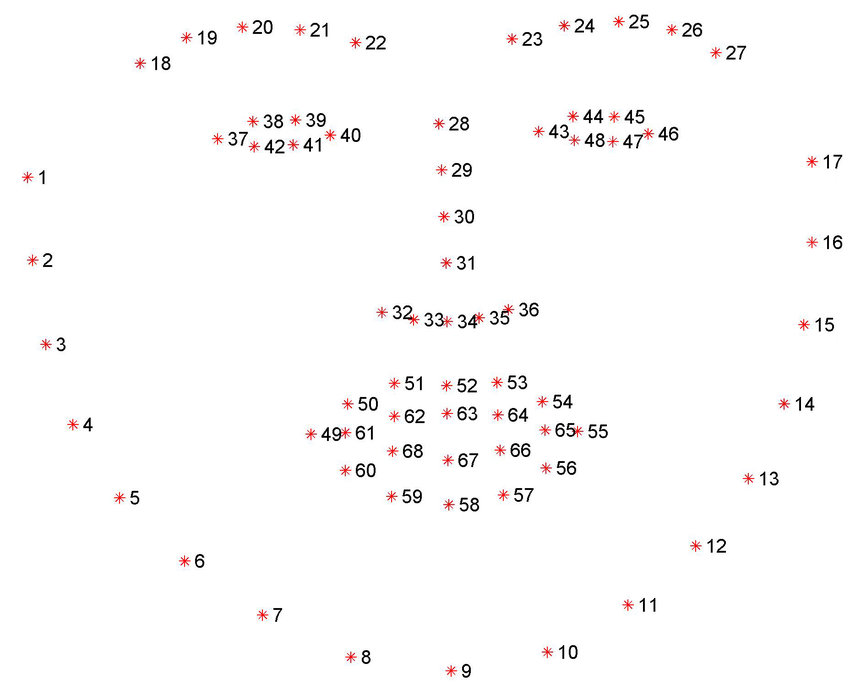
\includegraphics[width=\linewidth]{visual.png}
   \caption{Overview of the confusion matrix on the validation set.} 
   \label{fig:visual}
\end{figure}

\newpage

% \begin{itemize}
%   \item We collected datasets, preprocessed images or videos, 
%   and evaluated the training and testing data thoroughly from various public databases listed in.
%   \item To prepare training and testing images for loading we wrote a script.
%   \item All implemented classification models, such as VGG16, ResNet, 
%   or \textsc{GiMeFive} we built from scratch, 
%   and compared in accuracy in consideration of Layers and Architecture.
%   \item Subsequently optimization was executed with several techniques in a systematic manner. 
%   \item The classification scores of each emotion class, 
%   as well as the parameters to perform the confusion matrix heat map, 
%   are saved (in a serialised PyTorch state dictionary,) with respect to each image or video frame. 
%   \item We provide qualitative benefits such as interpretability to explain our model with Grad-CAM, 
%   combined with Face Landmarks 
%   Landmarks and the indication of the classified emotion percentages, 
%   emphasizing the main emotion.
%   \item To evaluate a video from a given video or live camera we created a script. 
% 	\item To illustrate the real-world performance of our best model \textsc{GiMeFive}, 
%   we edited and provide a demo video.
% \end{itemize}